\documentclass{bmstu}
\usepackage{multirow}
\newcolumntype{Y}{>{\centering\arraybackslash}X}

\bibliography{biblio}

\begin{document}
\def\labelitemi{--}
	
\setcounter{page}{3}
\maketableofcontents


\chapter*{ВВЕДЕНИЕ}
Во время выполнения выпускной квалификационной работы был разработан комбинированный алгоритм продвижения модельного времени.

Задача продвижения модельного времени является одной из важнейших задач имитационного моделирования \cite{imitation_modelling}, находящего применение во множестве областей в связи с дорогими или невозможными исследованиями реальных систем.

\chapter{Формальная постановка задачи}

IDEF0-диаграмма для комбинированного алгоритма продвижения модельного времени представлена на рисунках \ref{img:IDEF0-A0} \ref{img:IDEF0-A1}.

\begin{figure}[h!btp]
	\centering
	
\includegraphics[width=1\columnwidth]{inc/img/IDEF0-A0.png}
	\caption{IDEF0 нулевого уровня}
	\label{img:IDEF0-A0}	
\end{figure}

\begin{figure}[h!btp]
	\centering
	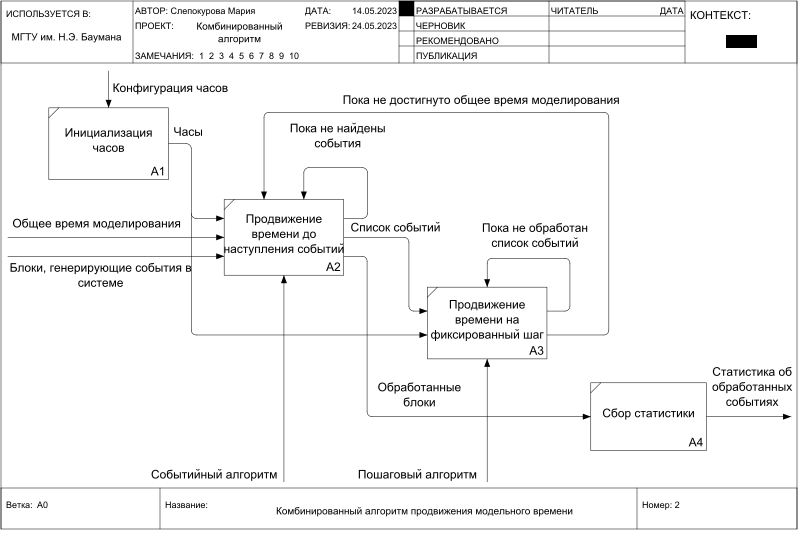
\includegraphics[width=1\columnwidth]{inc/img/IDEF0-A1.png}
	\caption{IDEF0 первого уровня}
	\label{img:IDEF0-A1}	
\end{figure}


\chapter{Разработанный алгоритм}
\section{Схема алгоритма}
На рисунке \ref{img:hybrid_simulate_schema} представлена схема комбинированного алгоритма продвижения модельного времени. 
\begin{figure}[h!btp]
	\centering
	\includegraphics[width=1\columnwidth]{inc/img/hybrid_simulate_schema.pdf}
	\caption{Схема комбинированного алгоритма}
	\label{img:hybrid_simulate_schema}	
\end{figure}

\clearpage
На рисунке \ref{img:hybrid_processLevel_schema} представлена схема алгоритма обработки одного уровня часов.
\begin{figure}[h!btp]
	\centering
	\includegraphics[width=1\columnwidth]{inc/img/hybrid_processLevel_schema.pdf}
	\caption{Схема алгоритма обработки одного уровня часовой структуры}
	\label{img:hybrid_processLevel_schema}	
\end{figure}

\clearpage
На рисунке \ref{img:hybrid_moveEvents_schema} представлена схема алгоритма перемещения событий из ячейки часовой структуры на уровень ниже.
\begin{figure}[h!btp]
	\centering
	\includegraphics[width=0.8\columnwidth]{inc/img/hybrid_moveEvents_schema.pdf}
	\caption{Схема алгоритма перемещения событий из ячейки часовой структуры на уровень ниже}
	\label{img:hybrid_moveEvents_schema}	
\end{figure}

\clearpage
На рисунке \ref{img:hybrid_processEvent_schema} представлена схема алгоритма обработки одного события.
\begin{figure}[h!btp]
	\centering
	\includegraphics[width=0.8\columnwidth]{inc/img/hybrid_processEvent_schema.pdf}
	\caption{Схема алгоритма обработки одного события}
	\label{img:hybrid_processEvent_schema}	
\end{figure}

\section{Описание реализации}

В листинге \ref{lst:DurationGenerator} представлен интерфейс \textbf{DurationGenerator}, который реализуют все классы-генераторы продолжительности, например, класс \textbf{UniformDurationGenerator}, представленный в листинге \ref{lst:UniformDurationGenerator}. Метод $generate$ класса \textbf{UniformDurationGenerator} используется для генерации продолжительности согласно равномерному распределению на основе значений $min$ и $max$, переданных в конструктор. Интерфейс \textbf{DurationGenerator} используется всеми сущностями, реализующими блоки системы, --- процессорами и генераторами, для генерации времени выполнения той или иной операции.
\listingfileKotlin{time/DurationGenerator.kt}{DurationGenerator}
\listingfileKotlin{time/UniformDurationGenerator.kt}{UniformDurationGenerator}

В листинге \ref{lst:Block} представлен интерфейс \textbf{Block}, который реализуют классы \textbf{Processor} и \textbf{Generator}. Метод $cleanupState$ используется для очищения всей статистики и текущего состояние блока. Метод $currentFinishTime$ --- метод-геттер, используемый для получения времени окончания текущего запущенного процесса. Метод $start$ используется для запуска процесса блока: для генератора --- процесса генерации заявки, для процессора --- процесса обработки заявки.
\listingfileKotlin{simulator/Block.kt}{Block}


В листинге \ref{lst:Event} представлен класс \textbf{Event}, описывающий события в моделируемой системе, где $time$ --- время наступления события, $block$ --- блок системы, сгенерировавший событие.
\listingfileKotlin{simulator/Event.kt}{Event}


В листинге \ref{lst:Request} представлен класс \textbf{Request}, описывающий заявки в моделируемой системе, где $timeIn$ --- время поступления заявки в с систему, $timeOut$ --- время выхода заявки из системы.
\listingfileKotlin{simulator/Request.kt}{Request}


В листинге \ref{lst:Processor} представлен класс \textbf{Processor}, описывающий блок процессора в моделируемой системе. Как уже было сказано выше, он реализует интерфейс \textbf{Block}. Рассмотрим подробнее поля класса:
\begin{itemize}
	\item $durationGenerator$ --- генератор продолжительности обработки заявки;
	\item $receivers$ --- список процессоров-получателей обработанной заявки;
	\item $queue$ --- очередь заявок процессора;
	\item $currentRequest$ --- текущая обрабатываемая заявка;
	\item $currentStartTime$ --- время начала обработки текущей заявки;
	\item $currentFinishTime$ --- время окончания обработки текущей заявки;
	\item $totalRequests$ --- общее количество обработанных заявок;
	\item $totalProcessingTime$ --- общее время работы процессора;
	\item $totalWaitingTime$ --- общее время ожидание заявок в очереди.
\end{itemize}
Помимо этого, класс \textbf{Processor} содержит вложенный класс \textbf{Statistics}, описывающий собираемую по процессору статистику --- общее количество обработанных заявок, среднее время обработки заявки и среднее время ожидания заявки в очереди. Статистика вычисляется с помощью метода $statistics$ на основе полученных за время моделирования значений $totalRequests$, $totalProcessingTime$, $totalWaitingTime$.
\listingfileKotlin{simulator/Processor.kt}{Processor}


В листинге \ref{lst:Generator} представлен класс \textbf{Generator}, описывающий блок генератора в моделируемой системе. Как уже было сказано выше, он реализует интерфейс \textbf{Block}. Рассмотрим подробнее поля класса:
\begin{itemize}
	\item $durationGenerator$ --- генератор продолжительности генерации заявки;
	\item $receivers$ --- список процессоров-получателей сгенерированной заявки;
	\item $currentRequest$ --- текущая генерируемая заявка;
	\item $currentStartTime$ --- время начала генерации текущей заявки;
	\item $currentFinishTime$ --- время окончания генерации текущей заявки;
	\item $totalRequests$ --- общее количество сгенерированных заявок;
	\item $totalGenerationTime$ --- общее время работы генератора.
\end{itemize}
Помимо этого, класс \textbf{Generator} содержит вложенный класс \textbf{Statistics}, описывающий собираемую по генератору статистику --- общее количество обработанных заявок и среднее время генерации заявки. Статистика вычисляется с помощью метода $statistics$ на основе полученных за время моделирования значений $totalRequests$, $totalGenerationTime$.
\listingfileKotlin{simulator/Generator.kt}{Generator}


В листинге \ref{lst:Simulator} представлен интерфейс \textbf{Simulator}, который реализуют классы-симуляторы для пошагового, событийного и комбинированного алгоритмов. В интерфейсе представлен вложенный класс \textbf{Statistics}, описывающий собираемую в процессе моделирования статистику. Класс содержит статистику, собранную со всех процессоров и генераторов, а также общее время выполнения симуляции.
\listingfileKotlin{simulator/Simulator.kt}{Simulator}


Листинг класса-симулятора \textbf{HybridSimulator}, реализующего комбинированный алгоритм продвижения модельного времени, приведен в приложении --- \ref{lst:full:HybridSimulator} 

\chapter*{ЗАКЛЮЧЕНИЕ}
\addcontentsline{toc}{chapter}{ЗАКЛЮЧЕНИЕ}
Было разработано программное обеспечение, демонстрирующее практическую осуществимость разработанного в ходе выполнения выпускной квалификационной работы комбинированного алгоритма продвижения модельного времени.


\makebibliography

\begin{appendices}
	\chapter{}
	\listingfileKotlin{simulator/HybridSimulator.kt}{full:HybridSimulator}
\end{appendices}


\end{document}